\chapter{BLAS}

\section{Datenstruktur für Matrizen}

Um vollbesetzte Matrizen zu speichern benötigt man eine Speicherfläche für alle Einträge der Matrix, Informationen wie die Einräge im Speicher organisiert sind und Informationen über die Größe der Matrix.

Es ist sinnvoll vollbesetzte Matrizen entweder Zeilen-der Matrix liegen hintereinander im Speicher oder Spaltenweise abzuspeichern.
Das bedeutet die Zeilen oder Spalten der Matrix liegen hintereinander im Speicher.
\begin{align*}
	A=
	\left(\begin{array}{ccc}
	a_{1,1} & a_{1,2} & a_{1,3} \\ 
	a_{2,1} & a_{2,2} & a_{2,3} \\ 
	a_{3,1} & a_{3,2} & a_{3,3} 
	\end{array} \right) \in \mathbb{R}^{m \times n}
\end{align*}
Matrix $A$ Zeilenweise gespeichert\\
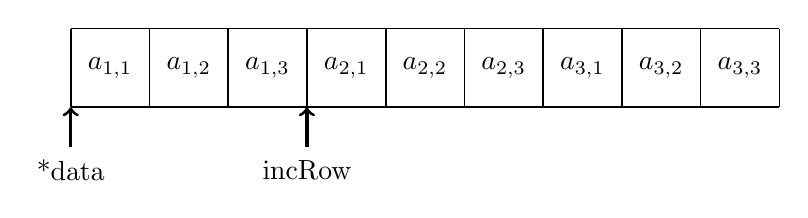
\begin{tikzpicture}
	\draw[semithick] (0,0) -- (9,0);
	\draw[semithick] (0,1) -- (9,1);
	\draw[semithick] (0,0) -- (0,1);
	\draw[semithick] (1,0) -- (1,1);
	\draw[semithick] (2,0) -- (2,1);
	\draw[semithick] (3,0) -- (3,1);
	\draw[semithick] (4,0) -- (4,1);
	\draw[semithick] (5,0) -- (5,1);
	\draw[semithick] (6,0) -- (6,1);
	\draw[semithick] (7,0) -- (7,1);
	\draw[semithick] (8,0) -- (8,1);
	\draw[semithick] (9,0) -- (9,1);
	
	\draw (0.5,0.5) node {$a_{1,1}$};
	\draw (1.5,0.5) node {$a_{1,2}$};
	\draw (2.5,0.5) node {$a_{1,3}$};
	\draw (3.5,0.5) node {$a_{2,1}$};
	\draw (4.5,0.5) node {$a_{2,2}$};
	\draw (5.5,0.5) node {$a_{2,3}$};
	\draw (6.5,0.5) node {$a_{3,1}$};
	\draw (7.5,0.5) node {$a_{3,2}$};
	\draw (8.5,0.5) node {$a_{3,3}$};
	
	\draw[->,line width=0.4mm] (0,-.5) -- (0,0);
	\draw (0,-0.8) node {*data};
	\draw[->,line width=0.4mm] (3,-.5) -- (3,0);
	\draw (3,-0.8) node {incRow};
\end{tikzpicture}\\
Matrix $A$ Spaltenweise gespeichert\\
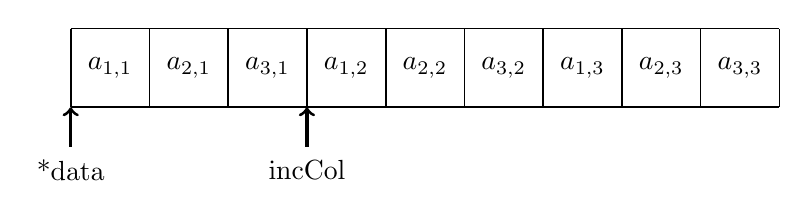
\begin{tikzpicture}
\draw[semithick] (0,0) -- (9,0);
\draw[semithick] (0,1) -- (9,1);
\draw[semithick] (0,0) -- (0,1);
\draw[semithick] (1,0) -- (1,1);
\draw[semithick] (2,0) -- (2,1);
\draw[semithick] (3,0) -- (3,1);
\draw[semithick] (4,0) -- (4,1);
\draw[semithick] (5,0) -- (5,1);
\draw[semithick] (6,0) -- (6,1);
\draw[semithick] (7,0) -- (7,1);
\draw[semithick] (8,0) -- (8,1);
\draw[semithick] (9,0) -- (9,1);

\draw (0.5,0.5) node {$a_{1,1}$};
\draw (1.5,0.5) node {$a_{2,1}$};
\draw (2.5,0.5) node {$a_{3,1}$};
\draw (3.5,0.5) node {$a_{1,2}$};
\draw (4.5,0.5) node {$a_{2,2}$};
\draw (5.5,0.5) node {$a_{3,2}$};
\draw (6.5,0.5) node {$a_{1,3}$};
\draw (7.5,0.5) node {$a_{2,3}$};
\draw (8.5,0.5) node {$a_{3,3}$};
	
\draw[->,line width=0.4mm] (0,-.5) -- (0,0);
\draw (0,-0.8) node {*data};
\draw[->,line width=0.4mm] (3,-.5) -- (3,0);
\draw (3,-0.8) node {incCol};
\end{tikzpicture}\\



Eine Datenstruktur benötigt ein Zeiger auf eine Speicherfläche, Informationen ob die Matrix Zeilen- oder Spaltenweise gespeichert ist und die Dimension der Matrix. 

So eine Datenstruktur könnte in C so aussehen.
\begin{lstlisting}
struct Matrix {
  double * data;
  std::ptrdiff_t incRow, incCol;
  std::size_t numRows, numCols;
}
\end{lstlisting}


Für Intel MKL und LAPACK Routinen müssen die Matrizen zeilenweise gespeichert.
\section{Einige Blasroutinen}


\subsection{Matrix-Matrix Produkt gemm}
\begin{align}
	C \leftarrow \beta * C + \alpha * A * B
\end{align}
\subsection{Matrix-Vector Produkt gemv}
\begin{align}
	y \leftarrow \alpha * A*x + \beta * y
\end{align}
\subsection{Rank1 update ger}
\begin{align}
	A \leftarrow A + \alpha * x * y^T
\end{align}

\subsection{Matrix-Matrix Produkt trmm}
\begin{align}
B \leftarrow  \alpha * op(A) * B \qquad \text{or} \qquad B \leftarrow  \alpha *  B * op(A)
\end{align}
\subsection{Matrix-Vector Produkt trmv}
\begin{align}
x \leftarrow \alpha * A*x \qquad \text{or} \qquad x \leftarrow \alpha * A^T*x
\end{align}

